\begin{SCfigure}
  \centering
  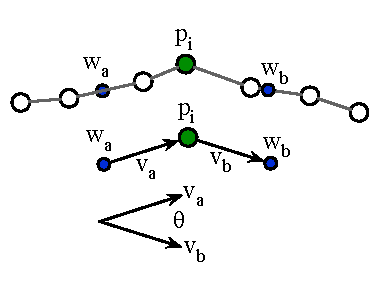
\includegraphics[width=3in]{img/curve-diagram.pdf}
  \caption[Curvature]{Illustration of how SIMI computes curvature
    about point $p_i$. Interpolated window boundary points $w_a$ and
    $w_b$ are equidistant (curvilinear-wise) from $p_i$ and are shown
    as dark dots. These window points let us create vectors $v_a$ and
    $v_b$. The curvature at $p_i$ is the signed angle between these
    vectors.}
  \label{fig:curvature-diagram}
\end{SCfigure}
